% This file was created by tikzplotlib v0.9.1.


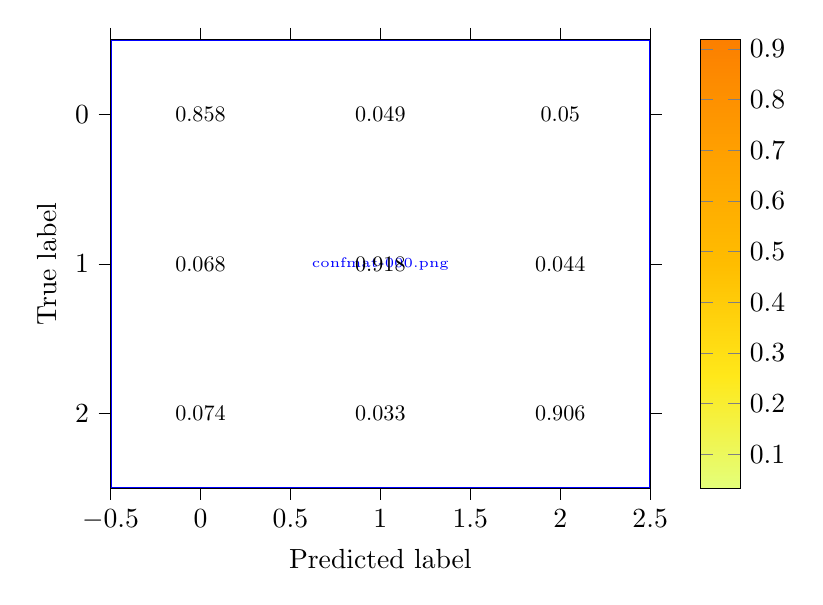
\begin{tikzpicture}

\begin{axis}[
colorbar,
colorbar style={ytick={0.1,0.2,0.3,0.4,0.5,0.6,0.7,0.8,0.9},yticklabels={\(\displaystyle 0.1\),\(\displaystyle 0.2\),\(\displaystyle 0.3\),\(\displaystyle 0.4\),\(\displaystyle 0.5\),\(\displaystyle 0.6\),\(\displaystyle 0.7\),\(\displaystyle 0.8\),\(\displaystyle 0.9\)},ylabel={}},
colormap={mymap}{[1pt]
  rgb(0pt)=(0.894117647058824,1,0.47843137254902);
  rgb(1pt)=(1,0.909803921568627,0.101960784313725);
  rgb(2pt)=(1,0.741176470588235,0);
  rgb(3pt)=(1,0.627450980392157,0);
  rgb(4pt)=(0.988235294117647,0.498039215686275,0)
},
point meta max=0.918,
point meta min=0.033,
tick align=outside,
tick pos=both,
x grid style={white!69.0196078431373!black},
xlabel={\(\displaystyle \mathrm{Predicted\ label}\)},
xmin=-0.5, xmax=2.5,
xtick style={color=black},
y dir=reverse,
y grid style={white!69.0196078431373!black},
ylabel={\(\displaystyle \mathrm{True\ label}\)},
ymin=-0.5, ymax=2.5,
ytick style={color=black}
]
\addplot graphics [includegraphics cmd=\pgfimage,xmin=-0.5, xmax=2.5, ymin=2.5, ymax=-0.5] {confmat-000.png};
\draw (axis cs:0,0) node[
  scale=0.8,
  text=black,
  rotate=0.0
]{0.858};
\draw (axis cs:0,1) node[
  scale=0.8,
  text=black,
  rotate=0.0
]{0.068};
\draw (axis cs:0,2) node[
  scale=0.8,
  text=black,
  rotate=0.0
]{0.074};
\draw (axis cs:1,0) node[
  scale=0.8,
  text=black,
  rotate=0.0
]{0.049};
\draw (axis cs:1,1) node[
  scale=0.8,
  text=black,
  rotate=0.0
]{0.918};
\draw (axis cs:1,2) node[
  scale=0.8,
  text=black,
  rotate=0.0
]{0.033};
\draw (axis cs:2,0) node[
  scale=0.8,
  text=black,
  rotate=0.0
]{0.05};
\draw (axis cs:2,1) node[
  scale=0.8,
  text=black,
  rotate=0.0
]{0.044};
\draw (axis cs:2,2) node[
  scale=0.8,
  text=black,
  rotate=0.0
]{0.906};
\end{axis}

\end{tikzpicture}
